

\section{\vta: An Algebra of \vita}\label{sec:vta}
We now discuss our visual text algebra, \vta, in detail.
We demonstrate how \vta captures various tasks in the usage example in Section~\ref{sec:example}
(see Figure~\ref{fig:fe},~\ref{fig:use-case-a}, and~\ref{fig:use-case-b}). 
%In this section, we first describe \vta's underlying data domain.
%We then define the current operators in \vta that enable users to specify various \vita workflows and interactions within \vita tools such as \system. 

%To the best of our knowledge, an algebra for \vita has never
% been defined previously. 
%However, our work draws inspiration from relational algebra~\cite{codd} and prior work on visualization grammars~\cite{satyanarayan2016vega,satyanarayan2015reactive,stolte2002polaris,bostock2009protovis,bostock2011d3}.


\subsection{\vta Specification}\label{sec:data_domain}
\stitle{Data domain.}
\vita involves many data types, including different forms of text (\eg words, tokens, sentences), complex data types like lists, vectors, and even visualizations. We define the data domain of \vita as $D = \{P, S\}$, where $P$ and $S$ are sets of primitive and synthesized (\ie composite) data types. The domains of primitive data types are taken from, $P = \{\alpha^*, \mathbf{int}, \mathbf{float}, \mathbf{bool}$,
$\mathbf{datetime},\mathbf{List}, \mathbf{Vector}, \mathbf{Dictionary}\}$. The domain $\alpha^*$ is the set of finite strings
over an alphabet $\alpha$. The domains of composite data types are taken from, $S = \{\mathbf{Text}$, $\mathbf{Visualizations}\}$. If a  schema of the data is not specified upfront, the data is initially assumed to be from the domain $\alpha^*$. Each domain $d_i \in D$ includes a generator function $g_i: \alpha^* \rightarrow d_i$ which defines the rule for inferring exact data types of the respective domain. For example, the composite $\mathbf{Text}$ data types (\eg words, tokens, sentences) are generated using a context free grammar~\cite{charniak1997statistical}. The generator function of visualization data types is defined based on Vega-Lite~\cite{satyanarayan2016vega}: $\mathbf{Visualizations} = (data, transforms, mark-type, encodings)$. \vta operators can be specified in a \emph{json} or as declarative commands that are available through a \vta library in Python.


% \candidate{We now explain how users specify \vita workflows in \vta.
% While explaining the algebra, we also demonstrate how \vta captures various tasks in the usage example in Section~\ref{sec:example}
% (see Figure~\ref{fig:fe},~\ref{fig:use-case-a}, and~\ref{fig:use-case-b}). As shown in these figures, \vta operators can be specified in a \emph{json} format or as declarative commands that are available through a \vta library in Python.}

\stitle{Selection operator.}
\vta enables the specification of interaction through selections. 
Selection operations select data points of interest on which subsequent operations in the workflow may be performed (\eg row(s) in Table View, visualization mark(s) in Visualization View). Supported selection types include a single point (\eg a table row, marks like a bar or a circle in a chart),
a list of points (\eg rows, bars, or circles), or an interval of points (\eg ten rows starting from row $i$, circles in scatterplot within $x$-axis range). The selection criteria are specified by a predicate to determine the set of selected points. \code{Filter} is an example of list selection where the selection predicate is the filtering condition. 
\vta also supports similar types of selections on visualizations (Figure~\ref{fig:use-case-b}a). Besides \emph{json} specification, users can also perform such selections by writing commands in Notebook View. For example, Figure~\ref{fig:fe}F shows how a user can select a bar (\eg the word ``comfy'') in the bar chart using a \vta command: 

% \begin{figure}[!htb] 
% \vspace{-10pt}
%   \centering
%   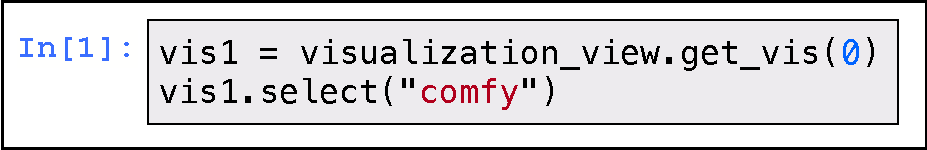
\includegraphics[width=\linewidth]{figures/notebook.pdf}
%   \caption{\small Selecting a bar chart element using \vta command.\label{fig:notebook}}
%  \vspace{-10pt}
% \end{figure}


\begin{figure*}[tbp]
\centering
\small
\begin{tabular}{ c c}
  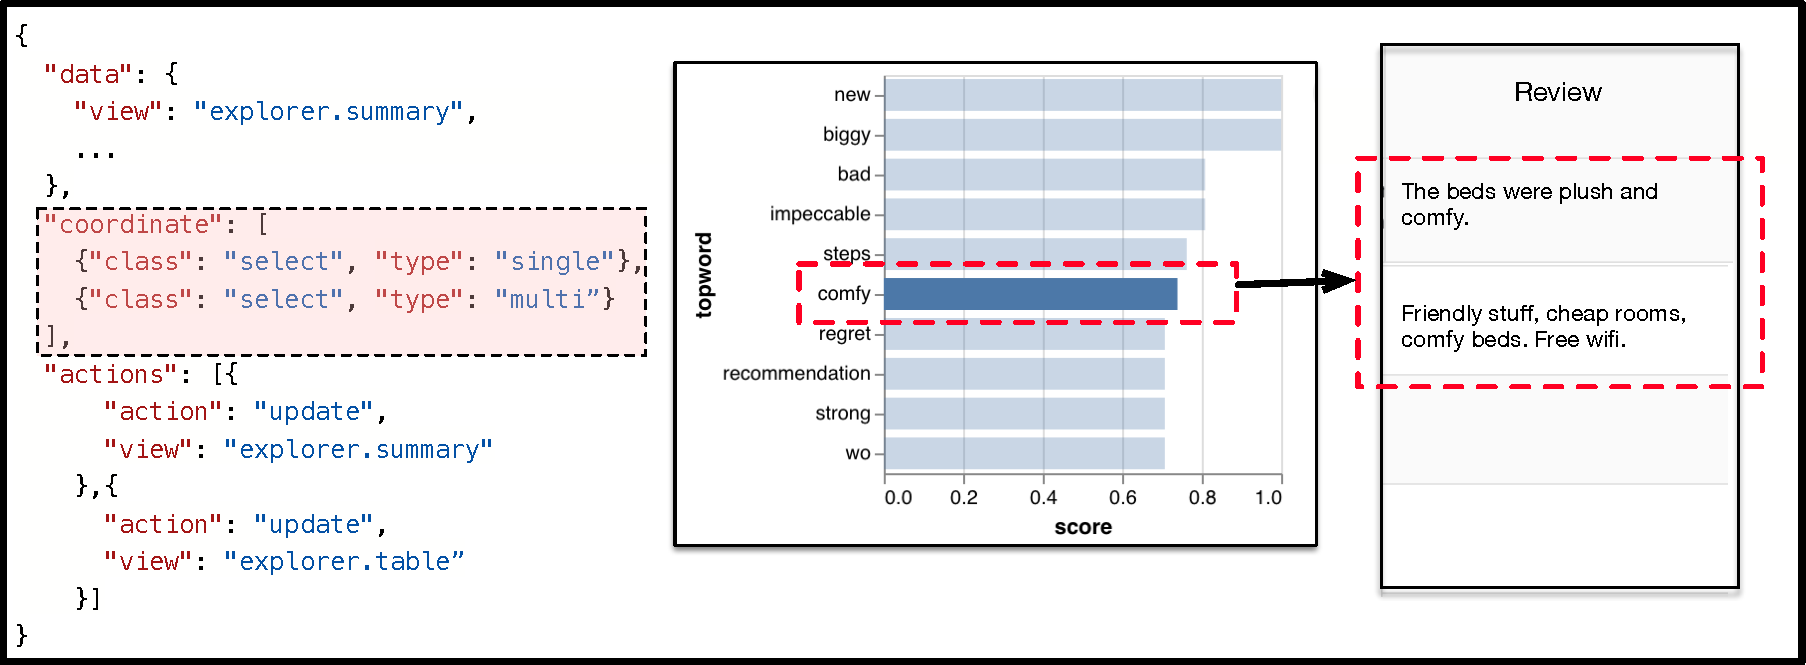
\includegraphics[width=0.5\linewidth,height=0.18\linewidth]{figures/unidirect_bar_table.pdf}   & 
  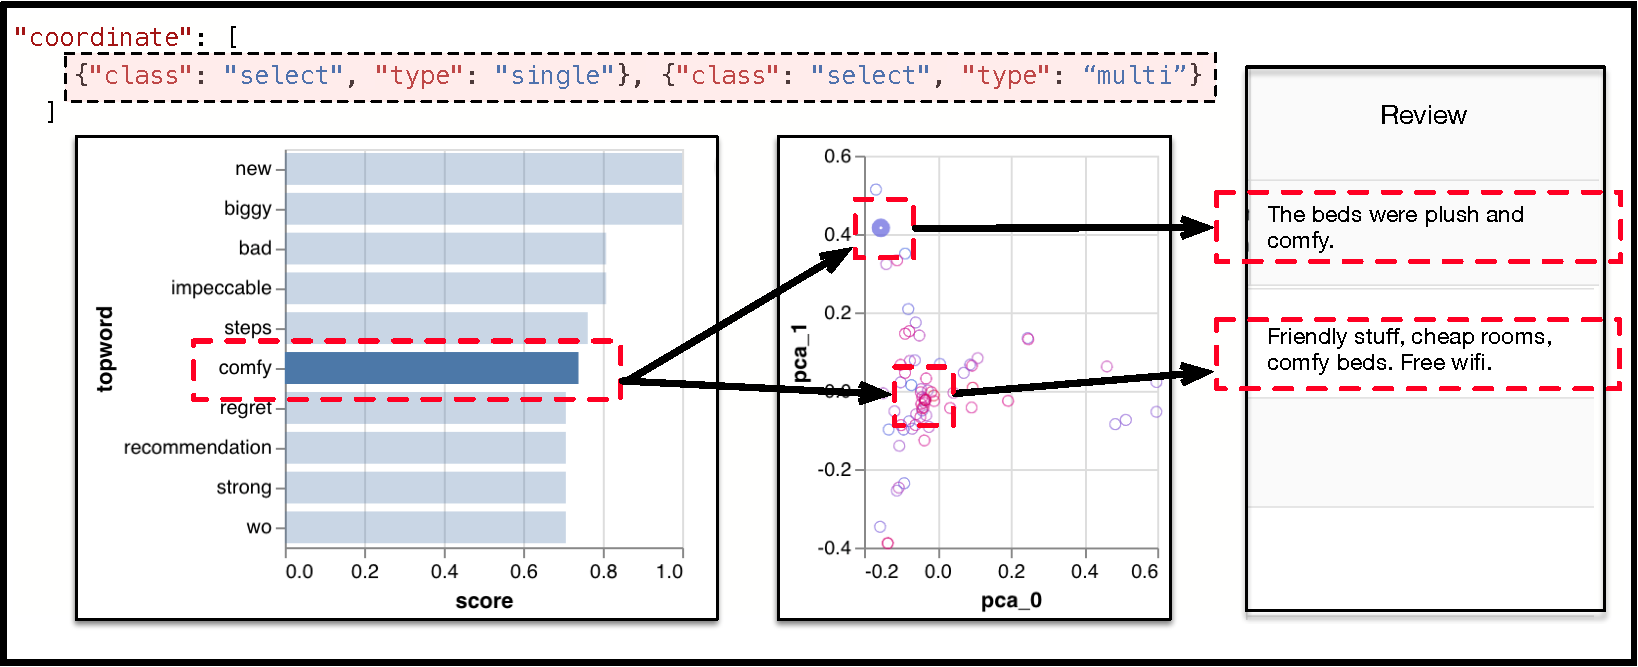
\includegraphics[width=0.5\linewidth,height=0.18\linewidth]{figures/unidirect_bar_table_scatter.pdf} \\
     (a) Coordination of two views & 
     (b) Coordination of three views 
\end{tabular}
    \caption{\small Multi-view coordination. (a) Use the \code{coordinate} operator to link the bar chart and Table View. Selecting a bar (word) in the bar chart triggers a \code{filter} by the selected word on Table View . (b) Coordinating the bar chart and scatterplot links the three views. Selecting a bar in the bar chart highlights relevant points in the scatterplot, and filters relevant rows in Table View.}
    \label{fig:use-case-b}
    \vspace{-15pt}
\end{figure*}

 %Multi-view coordination specification. (a) Use the \code{coordinate} operator to create a unidirectional coordination between the bar chart and Table View. Selecting a bar (word) in the bar chart triggers a \code{filter} operation on Table View by the selected word. (b) Creating a unidirectional coordination between the bar chart and scatterplot automatically links the three views (multi-view coordination). For the previous action on the bar chart, all relevant points in the scatterplot are selected, in addition to filtering Table View.

\stitle{Transformation operators.}
While developing \system, we identified a set of core transformation operators that encompasses the various \vita workflows. 
These transforms manipulate the
components of the selection they are applied to. 
Note that the core operator set is minimal, and there is room for adding more operators to make \vta more expressive (\textbf{D4}). 
The transformation operation has five subclasses: \code{project}, \code{mutate}, \code{aggregate}, \code{set}, and \code{visualize}. The \code{project} operators change the dimensionality (\eg LDA, PCA) or cardinality (\eg stopword removal) of the input data or update the content (\eg lowercase). The \code{mutate} operator generates a new representation of the input data (\eg create a list of tokens or feature vectors from text). The \code{aggregate} operator computes summary statistics of the input data (\eg average review length in a corpus). The \code{set} operations enable set-like operators on the input data (\eg get unique tokens in the corpus). The \code{visualize} operator generates visualizations of data. Figure~\ref{fig:use-case-a} captures the data preprocessing phase of the workflow discussed in Section~\ref{sec:example}. Ada first cleans the reviews using \code{project} operators (Figure~\ref{fig:use-case-a}a),then applies a \code{mutate} operator (\eg TF-IDF feature vector creations) to featurize the reviews (Figure~\ref{fig:use-case-a}b). Finally, Ada computes the average TF-IDF score of each word (\code{aggregate}) and visualizes the top ranking words (\code{visualize}) using a bar chart (Figure~\ref{fig:use-case-a}c). 

%\candidate{Each operation takes an input from the given data domain $D$ and generates an output that also belongs to the same domain $D$.
%An \emph{action} defines how the resulting output should be used. An action can be of three types: \code{add}, \code{create}, \code{update}. For add action, the output becomes meta-data of the input (\eg metadata of a \vitaframe column). For \code{create}, the output becomes part of the data the user directly operates on (\eg create a new \vitaframe column). For \code{update}, the output essentially replaces the input data (\eg update an existing \vitaframe column).}


\stitle{Composite Transforms.}
\vta currently supports two composite transforms that combine unit transformation operations: \code{combine} and \code{synthesize}. The \code{combine} operator enables users to specify an operation pipeline. In Figure~\ref{fig:use-case-a}a, a user combines two \code{project} operations with a \code{set} operation into a single operation. Similarly, in Figure~\ref{fig:use-case-a}c, a user combines \code{aggregate} and \code{visualize} operators into a single operation for bar chart creation. The \code{synthesize} operator enables users to create new operations from these combinations which can be reused later. For example, a user can \code{synthesize} the previous cleaning pipeline to be a \code{clean} operator which then becomes an operation in the \emph{Operator View} and is used later.




\subsection{Multi-view Coordination}
So far, we have explained selections that are defined within a single view. However, selections that involve multiple views cannot be captured by a single-view-based specification. We define a coordination operator called \code{coordinate} that captures multi-view coordination. For example, in Figure~\ref{fig:use-case-b}a, selecting a top-word bar in the bar chart filters relevant reviews in Table View (Visualization View $\rightarrow$ Table View coordination). The \code{coordinate} operator needs to also resolve the mapping between views and composite selections across views.

% \candidate{
% So far we have explained selections that are defined within a single view (\eg Table View or Visualization View). However, selections that involve multiple views cannot be captured by the default single-view-based \vta specification. We define a coordination operator called \code{coordinate} that captures such multi-view coordination.
% Coordination can be either unidirectional or bidirectional. For example, as shown in Figure~\ref{fig:use-case-b}a, selecting a top-word bar in the bar chart and filtering corresponding Table View rows is a unidirectional coordination (Visualization View $\rightarrow$ Table View). However, adding a selection in the reverse direction makes the coordination bidirectional. For example, changing opacity of the bars in the bar chart based on reviews selected in Table View. Currently, \system supports only unidirectional coordination within a single specification. To create a bidirectional specification, users are required to specify two unidirectional specifications. Besides the direction of coordination, the \code{coordinate} operator needs to resolve the mapping between coordinated views and composite selections across views.
% }

\stitle{Mapping coordination.} 
In Figure~\ref{fig:use-case-b}a, there is a one-to-many mapping from the bar chart to Table View---selecting a bar filters two that reviews contain the word in ``comfy''.
In Figure~\ref{fig:use-case-b}b, there is a one-to-many mapping from the bar chart to scatterplot and a one-to-one mapping from the scatterplot to Table View. Therefore, the \code{coordinate} operator needs to resolve the mapping among views, so that relevant visualization marks are selected/highlighted in respective views. Users can specify the mapping using the \emph{type} tag in respective \code{select} operators of the views. For example, in Figure~\ref{fig:use-case-b}a, the user selects type \emph{single} for the bar chart and \emph{multi} for Table View. 


% \candidate{
% \stitle{Mapping coordination.} 
% In Figure~\ref{fig:use-case-b}a, there is a one-to-many mapping from the bar chart to Table View---selecting a bar may filter multiple reviews that contain the top-word (\eg two reviews contain the word in ``comfy'').
% In Figure~\ref{fig:use-case-b}b, there is a one-to-many mapping from the bar chart to scatterplot and a one-to-one mapping from the scatterplot to Table View. Therefore, the \code{coordinate} operator needs to resolve the coordination mapping among views on the fly, so that relevant visualization marks are selected/highlighted in respective views. In our current \vta implementation,
% users are required to explicitly specify the mapping using the \emph{type} tag in respective \code{select} operators of the views. For example, in Figure~\ref{fig:use-case-b}a, the user selects type \emph{single} (\ie one) for the bar chart and \emph{multi} (\ie many) for Table View. 
% We aim to automate the mapping process in future by resolving the mapping between the underlying data of the respective views.}

\stitle{Resolving composite selections.}  
Users can add multiple single-view selections to a view. For example, in Figure~\ref{fig:use-case-b}b, the user adds a link from the bar chart to the scatterplot, which creates a multi-view coordination among the bar chart, scatterplot, and Table View.
Selecting a bar in the bar chart highlights multiple circles (scatterplot) and reviews (Table View). However, following the top-word selection, the user may select a rectangular area in the scatterplot or select multiple reviews in the table. Currently, \system only supports independent selection. We outline advanced composite specifications such as \code{union} and \code{intersection} as future work.

% \stitle{Resolving composite selections.}  
% Given a visualization, users can add multiple unidirectional coordinations to other views or visualizations. For example, in Figure~\ref{fig:use-case-b}b, the user adds a unidirectional coordination from the bar chart to the scatterplot which creates a multi-view coordination among the bar chart, scatterplot, and Table View.
% Selecting a bar in the bar chart highlights multiple circles (scatterplot) and reviews (Table View). However, following the top-word selection, the user may select a rectangular area in the scatterplot or select multiple reviews in the table. Currently, \system only supports independent selection. We outline advanced composite specifications such as \code{union} and \code{intersection} as future work.

% \saj{It is not clear whether we should deselect the previous selection and only highlight current selection in the scatterplot and update corresponding bar chart and table view selections, \ie always perform independent selection. The other option is to perform a \code{union} or \code{intersection} among the selected data points of all the selections}. 





% \section{\vta: An Algebra of \vita}\label{sec:vta}

% In this section, we first describe \vta's underlying data domain.
% We then define various operators in \vta that enable users to specify various \vita workflows and interactions within \vita tools such as \system. 
% To the best of our knowledge, an algebra for \vita has never
% been defined previously. 
% %However, our work draws inspiration from relational algebra~\cite{codd} and prior work on visualization grammars~\cite{satyanarayan2016vega,satyanarayan2015reactive,stolte2002polaris,bostock2009protovis,bostock2011d3}.

% \begin{figure*}[!htb]
% \centering
% \small
% \begin{tabular}{ c c c}
%   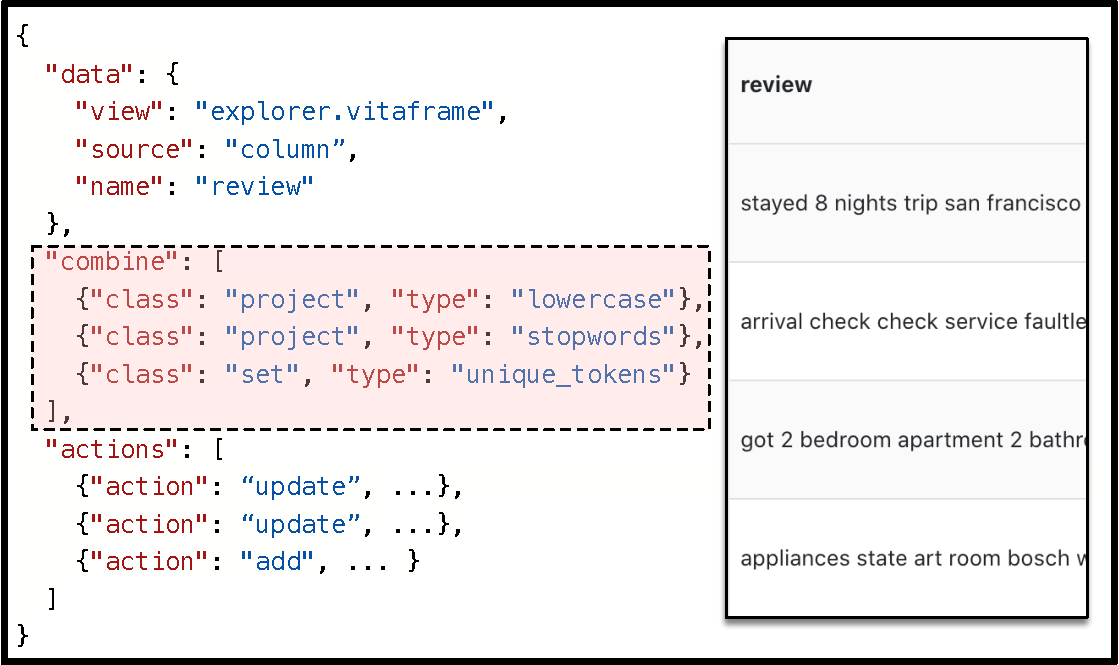
\includegraphics[width=0.3\linewidth,height=0.18\linewidth]{figures/combine_clean.pdf}   & 
%   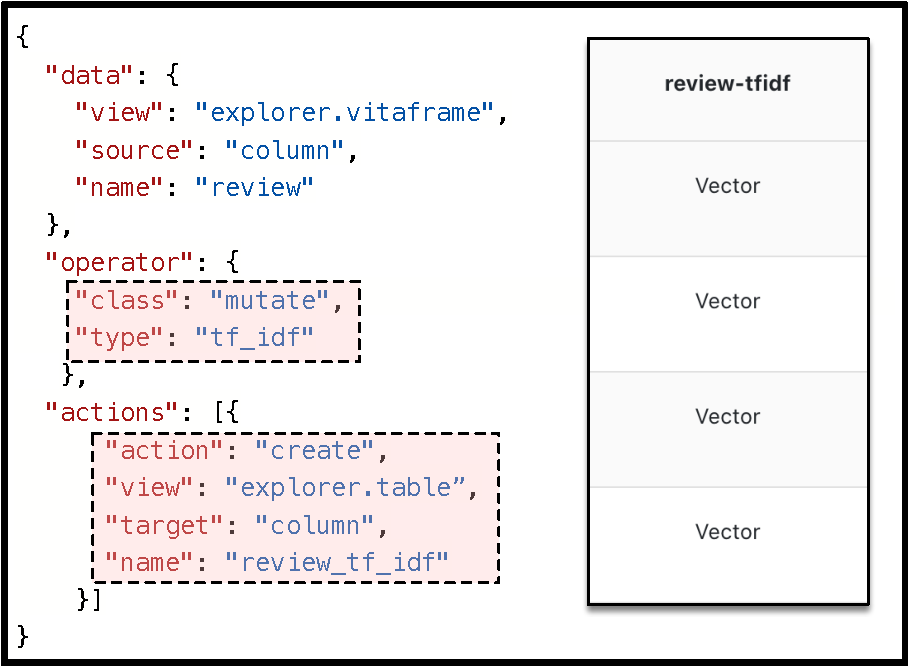
\includegraphics[width=0.3\linewidth,height=0.18\linewidth]{figures/tf_idf.pdf} & 
%   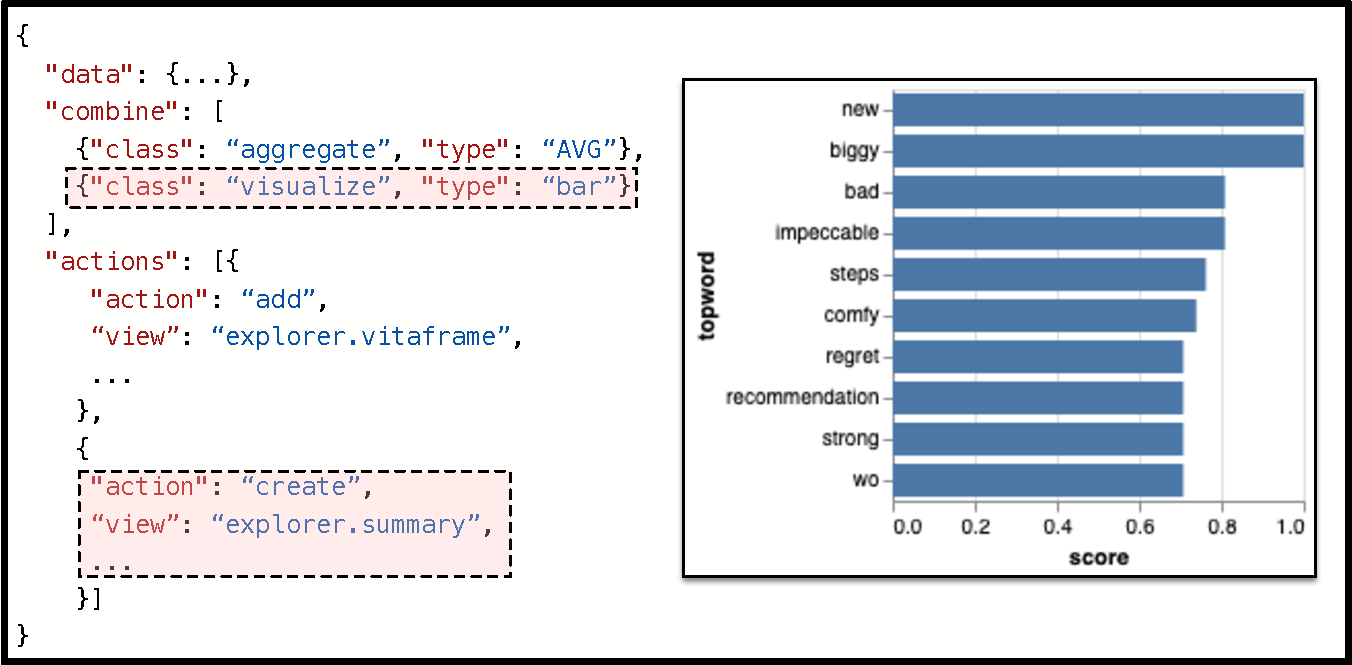
\includegraphics[width=0.4\linewidth,height=0.18\linewidth]{figures/barchart.pdf} \\
%      (a) Clean and generate metadata & 
%      (b) Create TF-IDF feature vector &
%      (c) Visualize top-words by TF-IDF score
% \end{tabular}
%     \caption{\small Example of \vta specification. (a) Use \code{combine} operator to clean data (\eg \code{lowercase}, \code{remove\_stopwords}) and generate metadata (\eg \code{unique\_token} to create token dictionary) for use in subsequent steps. (b) Define featurization operation and subsequent action of column creation in table view. (c) Compute the average TF-IDF score for each token in the dictionary using \code{aggregate} operator and then create a bar chart of top-ranked words using \code{visualize} operator.}
% \vspace{-15pt}
%     \label{fig:use-case-a}
% \end{figure*}

% \subsection{Data Domain Specification}\label{sec:data_domain}

% As explained earlier, \vita workflows handle various data types, from different forms of text strings like words, tokens (\eg cleaned words), sentences to more complex data types like lists, vectors, and even visualizations. We define the data domain of \vita as $D = \{P, S\}$, where $P$ and $S$ are sets of primitive and synthesized (\ie composite) data types. The domains of primitive data types are taken from, $P = \{\alpha^*, \mathbf{int}, \mathbf{float}, \mathbf{bool}$,
% $\mathbf{datetime},\mathbf{List}, \mathbf{Vector}, \mathbf{Dictionary}\}$. The domain $\alpha^*$ is the set of finite strings
% over an alphabet $\alpha$. The domains of composite data types are taken from, $S = \{\mathbf{Text}$, $\mathbf{Visualizations}\}$. If a  schema of the data is not specified upfront, the data is initially assumed to be from the domain $\alpha^*$. Each domain $d_i \in D$ includes a generator function $g_i: \alpha^* \rightarrow d_i$ which defines the rule for inferring exact data types of the respective domain. For example, the composite $\mathbf{Text}$ data types (\eg words, tokens, sentences) are generated using a context free grammar~\cite{charniak1997statistical}. The generator function of visualization data types is defined based on Vega-Lite~\cite{satyanarayan2016vega}: $\mathbf{Visualizations} = (data, transforms, mark-type, encodings)$.



% \subsection{Interaction Specification}
% To support various user interactions, a \vta specification may
% include a set of selections.
% Selections identify the set of data points a user is interested in manipulating in a given view (\eg table view, visualization view). In this section, we  define the selection operator, describe
% a series of transforms for modifying selections, discuss rules for creating composite transformations, and explain how coordination among views can be specified.
% While explaining the algebra, we also demonstrate how \vta captures various tasks in the usage example in Section~\ref{sec:example}
% (see Figure~\ref{fig:use-case-a},~\ref{fig:notebook}, and~\ref{fig:use-case-b}). As shown in these figures, \vta operators can be specified in either \emph{json} format or a declarative language.

% \subsubsection{Selection Operator}
% Selection operations select data points of interest on which subsequent operations in the workflow may be performed (\eg row(s) in the table view, visualization mark(s) in the visualization view). Supported selection types include a single point (\eg a table row, a mark like bar or a circle in a chart),
% a list of points (\eg rows, bars, or circles), or an interval of points (\eg 10 rows starting from row $i$, circles in scatterplot within $x$-axis range). The selection criteria is specified by a predicate to determine the set of selected points. \code{Filter} is an example of list selection where the selection predicate is the filtering condition. While not currently supported, sampling can be another selection operation where users may define a specific sampling criteria or provide a sampling function.
% Visualizations also support similar selections. For example, in Figure~\ref{fig:use-case-b}a, clicking a bar is a point selection. The corresponding \vta specification is highlighted in salmon color. Besides \emph{json} specification,
%  users can also perform such selections by writing commands in the notebook view. For example, Figure~\ref{fig:notebook} shows how a user can select a bar (\eg the word ``comfy'') in the bar chart using a \vta command: 
% \begin{figure}[!htb] 
% \vspace{-10pt}
%   \centering
%   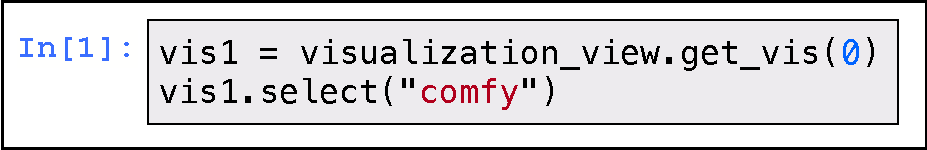
\includegraphics[width=\linewidth]{figures/notebook.pdf}
%   \caption{\small Selecting a bar chart element using \vta command.\label{fig:notebook}}
%  \vspace{-10pt}
% \end{figure}



% \subsubsection{Selection Transforms}
% While developing \system, we identified a set of core transformation operators that encompasses the various \vita workflows. 
% These transforms manipulate the
% components of the selection they are applied to. 
% Note that the core operator set is minimal and there is room for adding more operators to make \vta even more expressive (\textbf{D4}). 

% The transformation operation has five subclasses: \code{project}, \code{mutate}, \code{aggregate}, \code{set}, and \code{visualize}. Each subclass may contain several operations. The \code{project} operators change the dimensionality (\eg LDA, PCA) or cardinality (\eg stopword removal) of the input data or updates the content (\eg lowercase). The \code{mutate} operator generates a new representation of the input data (\eg tokenize a text string to list of tokens, create feature vectors from text). The \code{aggregate} operator computes summary statistics of the input data (\eg average review (text) length in the corpus). The \code{set} operations enable set-like operators on the input data (\eg get unique tokens in the corpus). The \code{visualize} operator generates visualizations of data. For example, in Figure~\ref{fig:use-case-a}, the user first updates (\eg cleans) the reviews using \code{project} operators (Figure~\ref{fig:use-case-a}a). The user then applies a \code{mutate} operator (\eg TF-IDF feature vector creations) to featurize the reviews (Figure~\ref{fig:use-case-a}b). The user computes the average TF-IDF score of each word (\code{aggregate}) next. Finally, the user visualizes the top ranking words (\code{visualize}) according to their TF-IDF score using a bar chart (Figure~\ref{fig:use-case-a}c). Each operation takes an input from the given data domain $D$ and generates an output that also belongs to the same domain $D$.
% %An \emph{action} defines how the resulting output should be used. An action can be of three types: \code{add}, \code{create}, \code{update}. For add action, the output becomes meta-data of the input (\eg metadata of a \vitaframe column). For \code{create}, the output becomes part of the data the user directly operates on (\eg create a new \vitaframe column). For \code{update}, the output essentially replaces the input data (\eg update an existing \vitaframe column).

% \stitle{Composite Transforms.}
% \label{sec:operator_combine}
% \vta supports a number of composite transforms by combining unit transformation operations. \vta currently supports two types of compositions: \code{combine} and \code{synthesize}. The \code{combine} operator enables users to specify an operation pipeline. In Figure~\ref{fig:use-case-a}a, a user combines two \code{project} operations (\eg \code{lowercase}, \code{remove\_stopwords}) with a \code{set} operation (\eg unique token generation) into a single operation. Similarly, in Figure~\ref{fig:use-case-a}c, a user combines \code{aggregate} and \code{visualize} operators into a single operation for bar chart creation. The \code{synthesize} operator enables users to create new operations from these combinations which can be reused later. For example, a user can \code{synthesize} the previous cleaning pipeline to be a \code{clean} operator which then becomes an operation in the \emph{Operator View} and is used later.

% \begin{figure*}[!htb]
% \centering
% \small
% \begin{tabular}{ c c}
%   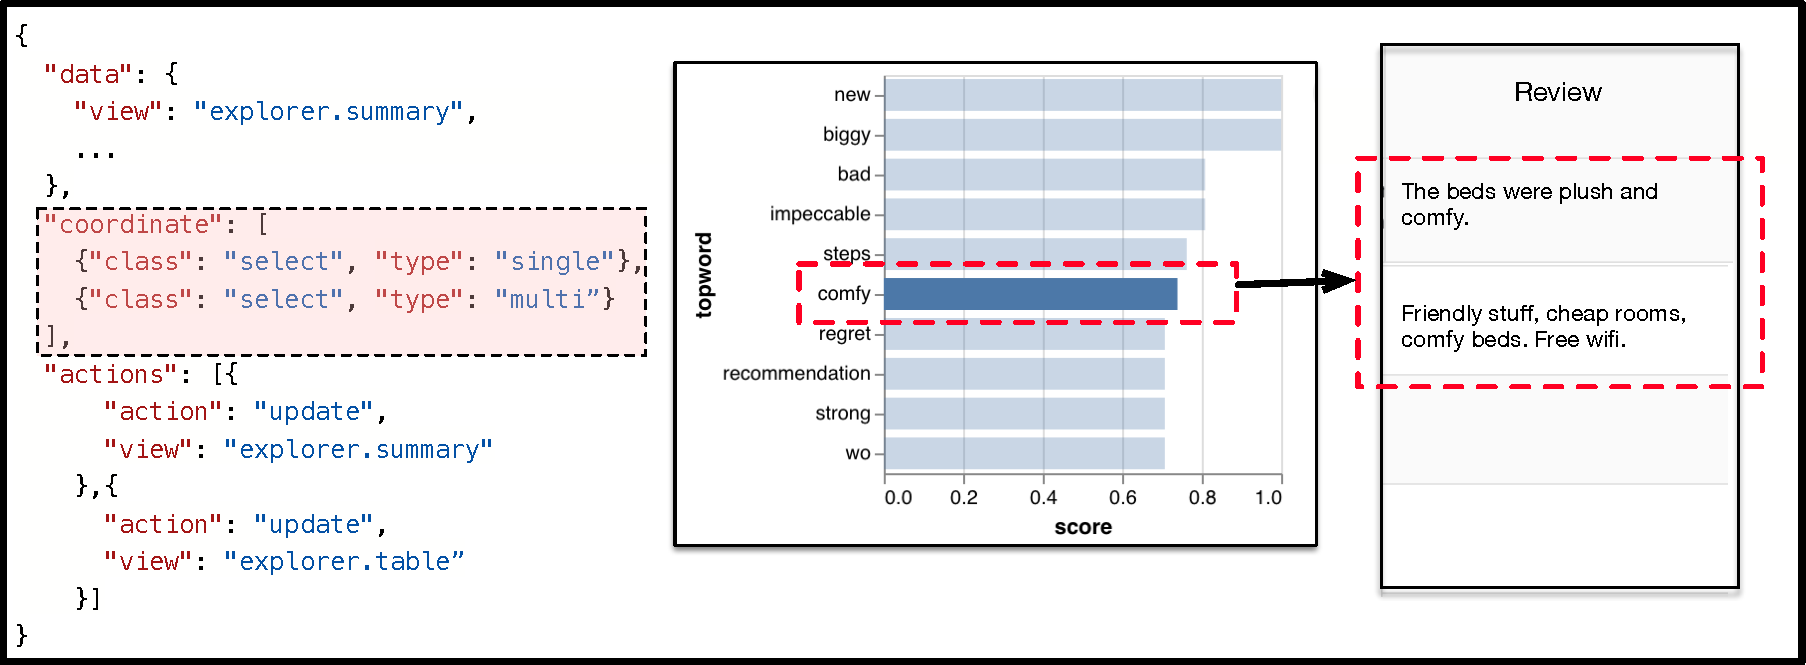
\includegraphics[width=0.5\linewidth,height=0.18\linewidth]{figures/unidirect_bar_table.pdf}   & 
%   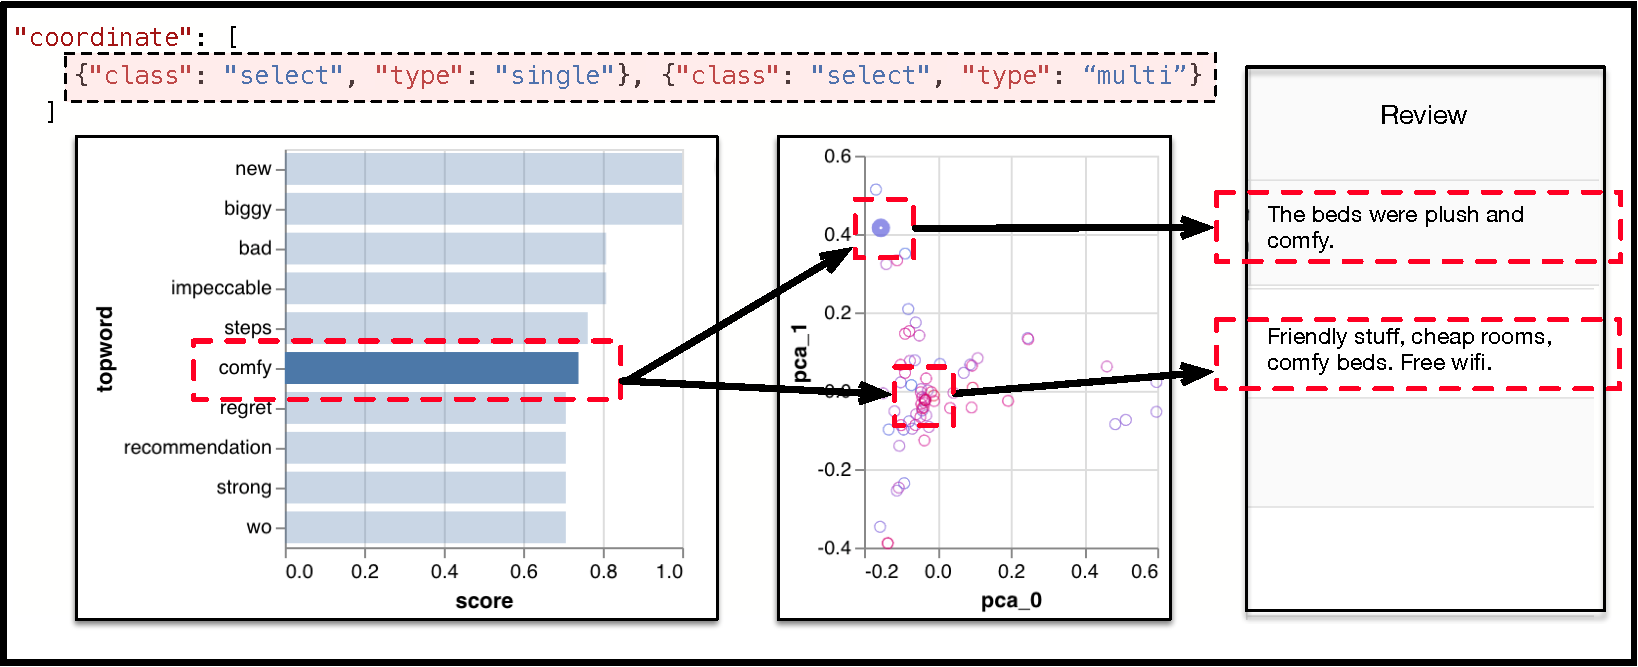
\includegraphics[width=0.5\linewidth,height=0.18\linewidth]{figures/unidirect_bar_table_scatter.pdf} \\
%      (a) Coordination of two views & 
%      (b) Coordination of three views 
% \end{tabular}
%     \caption{\small Example of enabling coordination among multiple views via \vta specification. (a) Use the \code{coordinate} operator to create a unidirectional coordination between the bar chart and table view. Selecting a bar (word) in the bar chart triggers a \code{filter} operation on the table view by the selected word. (b) Creating a unidirectional coordination between the bar chart and scatterplot automatically links the three views (multi-view coordination). For the previous action on the bar chart, all relevant points in the scatterplot are selected, in addition to filtering the table view.}
%     \label{fig:use-case-b}
%     \vspace{-15pt}
% \end{figure*}

% \subsubsection{Multi-view Coordination}
% So far we have explained selections that are defined within a single view (\eg table view or visualization view). However, selections that involve multiple views cannot be captured by the default single-view-based \vta specification. We define a coordination operator called \code{coordinate} that captures such multi-view coordination.
% Coordination can be either unidirectional or bidirectional. For example, as shown in Figure~\ref{fig:use-case-b}a, selecting a top-word bar in the bar chart and filtering corresponding table view rows is a unidirectional coordination (visualization view $\rightarrow$ table view). However, adding a selection in the reverse direction makes the coordination bidirectional. For example, changing opacity of the bars in the bar chart based on reviews selected in table view. Currently, \system supports only unidirectional coordination within a single specification. To create a bidirectional specification, users are required to specify two unidirectional specifications. \saj{Besides the direction of coordination, the \code{coordinate} operator needs to resolve the mapping between coordinated views and composite selections across views.}

% \stitle{Mapping coordination among views.} 
% \saj{For the coordination example in Figure~\ref{fig:use-case-a}a, there is a one-to-many mapping from the bar chart to the table view---selecting a bar may filter multiple reviews that contain the top-word (\eg two reviews contain the word in ``comfy'').
% In Figure~\ref{fig:use-case-b}b, there is a one-to-many mapping from the bar chart to scatterplot and a one-to-one mapping from the scatterplot to table view. Therefore, the \code{coordinate} operator needs to resolve the coordination mapping among views on the fly, so that relevant visualization marks are selected/highlighted in respective views. In out current \vta implementation,
% users are required to explicitly specify the mapping using the \emph{type} tag in respective \code{select} operators of the views. For example, in Figure~\ref{fig:use-case-b}a, the user selects type \emph{single} (\ie one) for the bar chart and \emph{multi} (\ie many) for table view. We aim to automate the mapping process in future by resolving the mapping between the underlying the data of the respective views.}

% \stitle{Resolving composite selections.}  
% Given a visualization, users can add multiple unidirectional coordinations to other views or visualizations. \saj{For example, in Figure~\ref{fig:use-case-b}b, the user adds a unidirectional coordination from the bar chart to the scatterplot which creates a multi-view coordination among the bar chart, scatterplot, and table view.
% Selecting a bar in the bar chart highlights multiple circles (scatterplot) and reviews (table view).} However, following the top-word selection, the user may select a rectangular area in the scatterplot or select multiple reviews in the table. \saj{It is not clear, whether we should deselect the previous selection and only highlight current selection in the scatterplot and update corresponding bar chart and table view selections, \ie always perform independent selection. The other option is to perform a \code{union} or \code{intersection} among the selected data points of all the selections}. Currently, \system only supports independent selection. We outline such advanced composite specifications (\eg \code{union} or \code{intersection} of selections) as future work.

% \hide{\subsection{\vital: The \vta specification language}
% \saj{While the \vta specifications make it easier to parse and execute \vita workflows in \system compiler, the \emph{json}-style specifications can be difficult for the users to compose. Moreover, such specification format diverges from the popular REPL-style specifications used in \vita workflows (\eg in computational notebooks). Therefore, we propose the development of \vital, a python-style declarative specification language that end-users can specify in the notebook view. Currently, we are at the early stage of \vital development that supports all of the aforementioned \vta operators. Since all operations belong to an operator subclass and all subclasses can be mapped to a high-level operator class, \vital specifications are similar to typical object oriented declarative languages. For example, to tokenize a \vitaframe column a user can first assign the column to a temporary variable ($col = VF.get_column('review')$) and then perform tokenization ($transformation.mutate.tokenize(col)$). The \vital specification translated to a \vta specification before compilation.
% Note that developers of  \vita systems like \system, are still required to use \emph{json}-style specification to define interactions within and among various components.}}


% \section{\vta: a grammar of \vita}
% \label{sec:vta}
% In this section, we first describe \vta's underlying data domain.
% We then define various operators in \vta that enables users to specify various \vita workflows and interactions within \vita tools such as \system. 
% To the best of our knowledge, an algebra for \vita has never
% been defined previously. However, our work takes inspiration from relational algebra~\cite{codd} and the grammar of graphics and visual interaction~\cite{satyanarayan2016vega,satyanarayan2015reactive,stolte2002polaris,bostock2009protovis,bostock2011d3}.


% \subsection{Data Domain Specification}
% \label{sec:data_domain}
% As explained earlier, \vita workflows handle various data types, from different forms of text strings like words, tokens (\eg cleaned words), sentences to more complex data types like lists, vectors, and even visualizations. We define the data domain of of \vita as $D = \{P, S\}$, where $P$ and $C$ are sets of primitive and synthesized (\ie composite) data types. The domains of primitive data types are taken from, $P = \{\alpha^*, \mathbf{int}, \mathbf{float}, \mathbf{bool}$,
% $\mathbf{List}, \mathbf{Vector}, \mathbf{Dictionary}, \mathbf{datetime}\}$. The domain $\alpha^*$ is the set of finite strings
% over an alphabet $\alpha$. The domains of composite data types are taken from, $S = \{\mathbf{Text}$, $\mathbf{Visualizations}\}$. If a  schema of the data is not specified upfront, the data is initially assumed to be from the domain $\alpha^*$. Each domain $d_i \in D$ includes a \emph{generator} function $g_i: \alpha^* \rightarrow d_i$ which defines the rule for inferring exact data types of the respective domain. For example, the composite $\mathbf{Text}$ data types (\eg words, tokens, sentences) are generated using a context free grammar~\cite{charniak1997statistical}. The generator function of visualization data types is defined based on the grammar of graphics outlined in Vega-Lite~\cite{satyanarayan2016vega}: $\mathbf{Visualizations} = (data, transforms, mark-type, encodings)$.

% \begin{figure*}[!htb]
% \centering
% \begin{tabular}{ c c}
%   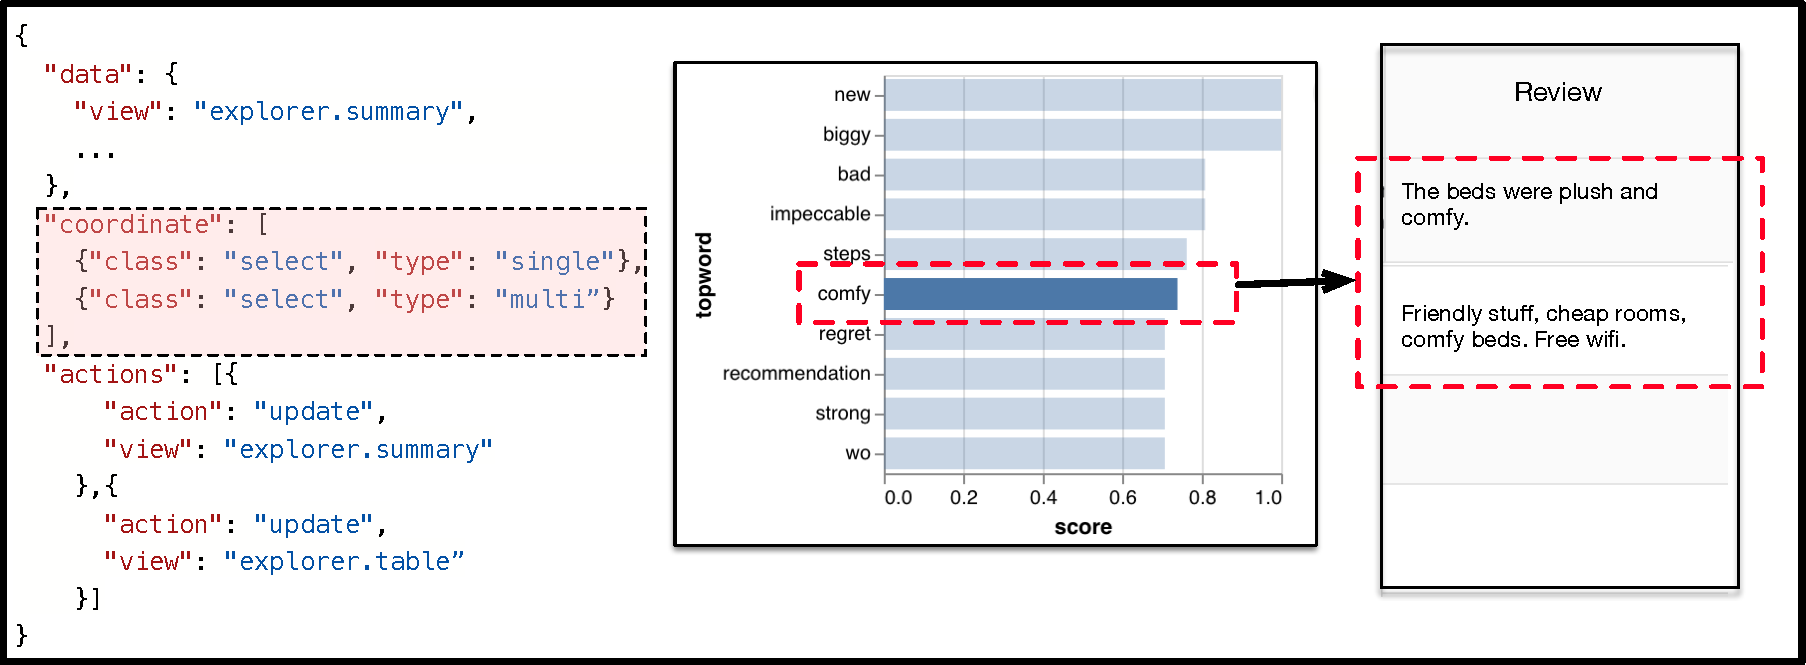
\includegraphics[width=0.5\linewidth,height=0.18\linewidth]{figures/unidirect_bar_table.pdf}   & 
%   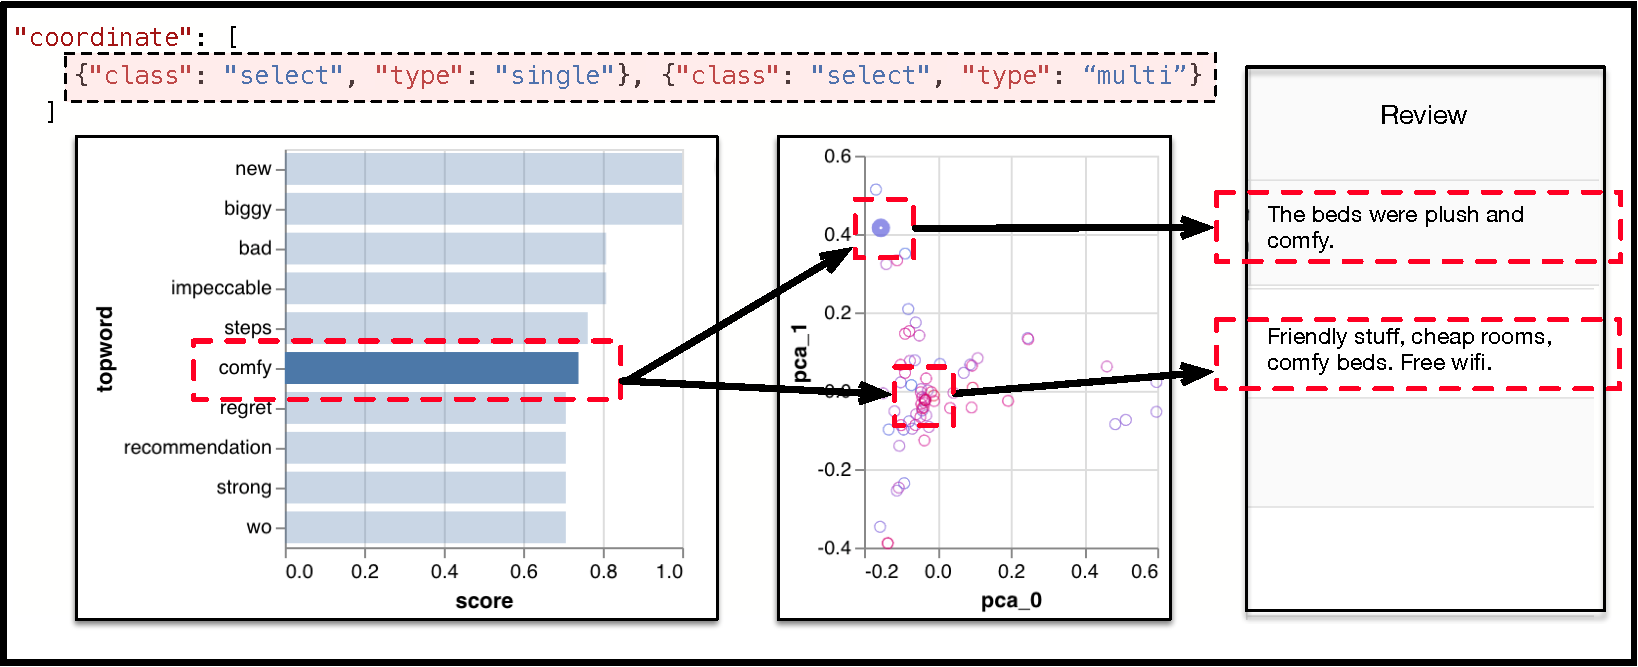
\includegraphics[width=0.5\linewidth,height=0.18\linewidth]{figures/unidirect_bar_table_scatter.pdf} \\
%      (a) Coordination of two views & 
%      (b) Coordination of three views 
% \end{tabular}
%     \caption{\small Example of enabling coordination among multiple views via \vta specification. (a) Use \emph{coordinate} operator create a unidirectional coordination between the bar chart and table view. Clicking a bar (word) in the bar chart triggers a \emph{filter} operation on the table view by the selected word. (b) Creating a unidirectional coordination between the bar chart and scatterplot automatically links the three views. For the previous action on the bar chart, all relevant points in the scatterplot (\ie multi-select event) are selected, in addition to filtering the table view.}
%     \label{fig:use-case-b}
%     \vspace{-15pt}
% \end{figure*}

% \subsection{The \vta Grammar of Interaction}
% To support various user interactions, a \vta specification may
% include a set of selections.
% Selections identify the set of data points a user is interested in manipulating in a given view (\ie table view, visualization view). In this section, we  define the selection operator, describe
% a series of transforms for modifying selections, discuss rules for creating composite transformations, and explain how coordination among views can be specified.
% While explaining the grammar, we also demonstrate how \vta captures various tasks in the usage example in Section~\ref{sec:example}
% (see Figure~\ref{fig:use-case-a} and~\ref{fig:use-case-b}). As shown in both of these figures, \vta specifications are expressed in \emph{json} format.

% \stitle{Selection Operator}
% Selection operations select data points of interest on which subsequent operations in the workflow may be performed (\eg row(s) in the table view, visualization mark(s) in the visualization view). Supported selection types include a single point (\eg a table row, a mark like bar or a circle in a chart),
% a list of points (\eg rows, bars, or circles), or an interval of points (\eg 10 rows starting from row $i$, circles in scatterplot within $x$-axis range). The selection criteria is specified by a \emph{predicate} to determine the set of selected points. \emph{Filter} is an example of \emph{list} selection where the selection predicate is the filtering condition. While not currently supported, we propose \emph{sampling} as another example of the selection class where users may define a specific sampling criteria or provide a sampling function.
% Visualizations also support similar selections. For example, in Figure~\ref{fig:use-case-b}a, clicking a bar is a \emph{point} selection. The corresponding \vta specification is highlighted in salmon color.



% \stitle{Selection Transforms}
% While developing \system, we discovered that there exists a set of core transformation operators that encompasses the various \vita workflows. 
% These transforms manipulate the
% components of the selection they are applied to. 
% Note that the core operator set is minimal and there is room for adding more operators to make the core collection even more expressive (\textbf{D4});
% in Figure~\ref{fig:use-case-a} and~\ref{fig:use-case-b}, we demonstrate 
% how a number of tasks in the use-case explained in Section~\ref{sec:example} are specified using \vta. 

% The transformation operator has five subclasses: \emph{project}, \emph{mutate}, \emph{aggregate}, \emph{set}, and \emph{visualize}. Each operator subclass may contain several operations. Project operators change the dimensionality (\eg LDA, PCA) or cardinality (\eg stopword removal) of the input data or updates the content (\eg lowercase). Mutate operator generates a new representation of the input data (\eg tokenize a text \emph{string} to \emph{list} of tokens, create feature vectors from text). Aggregate operator computes summary statistics of the input data (\eg average review (text) length in the corpus). Set operations enable set-like operators on the input data (\eg get unique tokens in the corpus). For example, in Figure~\ref{fig:use-case-a}, the user first updates (\ie cleans) the reviews using project operators (Figure~\ref{fig:use-case-a}a). The user then applies mutate operator (\ie TF-IDF feature vector creations) to featurize the reviews (Figure~\ref{fig:use-case-a}b). The user computes the average TF-IDF score of each word (\ie aggregate) next. Finally, the user visualizes the top raking words (\ie visualize) according to their TF-IDF score using a bar chart (Figure~\ref{fig:use-case-a}c).

% Each operation takes an input from the given data domain $D$ and generates an output that also belongs to the same domain $D$.
% An \emph{action} defines how the resulting output should be used. An action can be of three types: \emph{add}, \emph{create}, \emph{update}. For add action, the output becomes meta-data of the input (\eg metadata of a \vitaframe column). For create action, the output becomes part of the data the user directly operates on (\eg create a new \vitaframe column). For update action, the output essentially replaces the input data (\eg update an existing \vitaframe column).

% \stitle{Composite Transforms}
% \label{sec:operator_combine}
% \vta supports a number of composite transforms by combining unit transformation operations. Currently, \vta supports two types of compositions: \emph{combine} and \emph{synthesize}. Combine operator enables users to specify an operation pipeline. For example, in Figure~\ref{fig:use-case-a}a, a user combines two project operations (\ie lowercasing, stopwords removal) along with a set operation (\ie unique token generation) into a single operation. Similarly, in Figure~\ref{fig:use-case-a}c, a user combines aggregate and visualize operators into a single operation for bar chart creation. Synthesize operator enables users to create new operations from these combinations which can be reused later. For example, user can define the previous cleaning pipeline to be synthesized as a \emph{clean} operator which then becomes an operation in the \emph{Operator View} that the user can reuse later.



% \stitle{Coordination: Resolving Composite Selections}
% So far we have explained selections that are defined within a single view (\eg table view or visualization view). However, selections that involve multiple views cannot be captured by the default single-view-based \vta specification. We define a coordination operator called \emph{coordinate} that captures such multi-view coordination.
% Coordination can be either unidirectional or bidirectional. For example, as shown in Figure~\ref{fig:use-case-b}a, selecting a top-word bar in the bar chart and filtering corresponding table view rows is a unidirectional coordination (visualization view $\rightarrow$ table view). However, adding a selection in the reverse direction makes the coordination bidirectional. For example, changing opacity of the bars in the bar chart based on reviews selected in table view. Currently, \system supports only unidirectional coordination within a single specification. To create a bidirectional specification, users are required to specify two unidirectional specifications.

% Coordination operations can be more complex.
% Given a visualization, users can add multiple unidirectional coordinations to other views or visualizations. For example, in Figure~\ref{fig:fe}, there is scatterplot visualization in the visualization view. 
% Besides coordinating the table view filter with bar chart selection, a natural unidirectional coordination from the bar chart to the scatterplot is to highlight relevant reviews (circles) that contain selected top-word(s) (see Figure~\ref{fig:use-case-b}b). However, right after the top-word selection, the user may select another circle in the scatterplot or select multiple reviews in the table. It is not clear, whether we should deselect the previous selection in the scatterplot (\ie allow only \emph{single event selection}) along with the bar chart bar and table view rows or perform selection based on \emph{union} or \emph{intersection} of data points in other views that satisfy subsequent selections (\emph{multi-event selection}). Currently, \system only supports \emph{single event selection}. We outline bidirectional coordination specification along with more advanced composite specifications (\eg \emph{union} or \emph{intersection} of selections) as future work.

% \hide{\subsection{\vital: The \vta specification language}
% \saj{While the \vta specifications make it easier to parse and execute \vita workflows in \system compiler, the \emph{JSON}-style specifications can be difficult for the users to compose. Moreover, such specification format diverges from the popular REPL-style specifications used in \vita workflows (\eg in computational notebooks). Therefore, we propose the development of \vital, a python-style declarative specification language that end-users can specify in the notebook view. Currently, we are at the early stage of \vital development that supports all of the aforementioned \vta operators. Since all operations belong to an operator subclass and all subclasses can be mapped to a high-level operator class, \vital specifications are similar to typical object oriented declarative languages. For example, to \emph{tokenize} a \vitaframe column a user can first assign the column to a temporary variable ($col = VF.get_column('review')$) and then perform tokenization ($transformation.mutate.tokenize(col)$). The \vital specification translated to a \vta specification before compilation.
% Note that developers of  \vita systems like \system, are still required to use \emph{JSON}-style specification to define interactions within and among various components.}}



